\chapter{Exciton-polariton condensation in artificial lattices: An introduction}\label{CHONE}
In the last three decades, a two-dimensional system with strong light-matter interaction called a semiconductor microcavity has become a platform to observe Bose--Einstein condensation (BEC) in condensed matter physics.
The emergence of exciton-polaritons is the result of strong coupling between quantum well (QW) excitons and cavity photons in such semiconductor microcavities.
These quasi-particles were first predicted by Hopfield~\cite{Hopfield:1958aa} in the context of bulk semiconductors as the new eigenstates of a light-crystal Hamiltonian.
In 1992, the first experimental observation~\cite{Weisbuch:1992aa} of the strong coupling between excitons and photons in semiconductor microcavities was reported.

In 1996, it was proposed that in the ground state of the lower branch of exciton-polariton dispersion, quasi-BEC can form~\cite{Imamogu:1996aa}.
This prediction was later corroborated by several experimental works~\cite{Deng:2002aa,Kasprzak:2006aa,Balili:2007aa}.
Compared to conventional exciton BEC~\cite{Hanamura:1977aa} and cold atom BEC~\cite{Davis:1995aa,Pethick:2002tn}, polariton condensates have several advantages in different aspects.
%
\begin{itemize}
    \item \textit{Effective mass.}
In the vicinity of the ground state, the effective mass of polaritons is four orders of magnitude smaller than the mass of bare excitons.
This means that the critical temperature of the BEC for polaritons can be four orders of magnitude higher than the critical temperature of excitons~\cite{Pethick:2002tn}.
    \item \textit{Coherence.}
Due to the photonic component, polaritons can easily extend a coherent wave function in space despite the presence of crystal defects and disorder, which in the case of excitons can be easily localized.
    \item \textit{Lifetime.}
The lifetime of the polaritons ranges between $1$--$30$ ps~\cite{Wertz:2010aa} and up to $300$ ps~\cite{Sun:2017aa} with different Q factors of cavities and pumping in different materials.
This dynamical nature of the polariton condensates provides an experimental platform to study not only standard BEC physics but also non-equilibrium open systems consisting of highly degenerate interacting boson gases.
In contrast to equilibrium condensation, where only the lowest energy state can be macroscopically occupied, polaritons can form condensation in different states.
    \item \textit{Measurement.}
Experimentally, microcavity polaritons are one of the most accessible BEC systems.
This is because there is a one-to-one correspondence between the polaritons in mode $k_\parallel$ and the wavefunction of the emitted photon.
\end{itemize}
%

In the coming sections in this chapter, we will discuss some basic concepts about exciton-polaritons in BEC systems.
In Section~\ref{se:Ch1_microcavity_and_cp}, we will give a brief introduction to microcavities and cavity photons.
In Section~\ref{se:CH1_qw_ex}, we will discuss excitons, which are the matter part of polaritons, and then in Section~\ref{se:CH1_ex_pl} we will briefly review the basic properties of exciton-polaritons.
Last, we will discuss polariton condensates in Section~\ref{se:CH1_EP-BEC}.


\section{Microcavities and cavity photons}\label{se:Ch1_microcavity_and_cp}
%
\begin{figure}[ht]
    \centering
    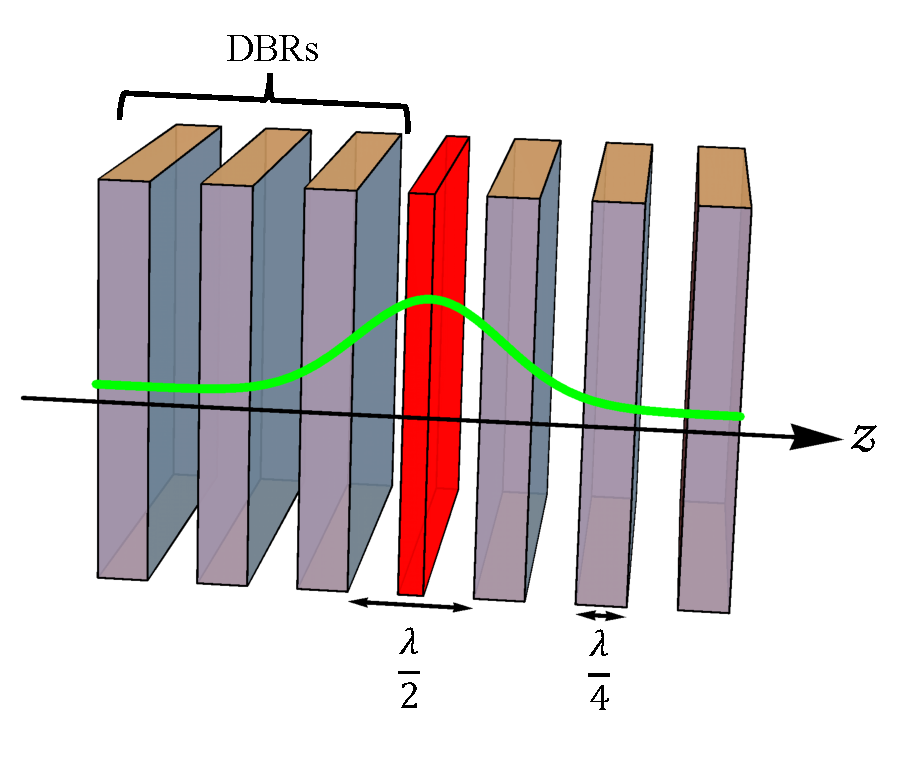
\includegraphics[width=0.55\linewidth]{Fig/Ch1/cavity3D.pdf}
    \caption[Microcavity schematic]{Schematic for a cavity along the $z$ direction. A cavity of thickness $\frac{\lambda}{2}$ is sandwiched by distributed Bragg reflectors (DBRs) of thickness $\frac{\lambda}{4}$. The QW is in the middle of the cavity (red). Light intensity (green curve) indicates that the cavity photons are localized inside the cavity.}
    \label{fig:Ch1_cavity}
\end{figure}
In Fig.~\ref{fig:Ch1_cavity}, we show a typical semiconductor microcavity structure.
% A thickness of $\frac{\lambda}{2}$ cavity layer contained QWs is sandwiched between two distributed Bragg reflectors (DBRs).
The semiconductor QW is located in the middle of the cavity between two distributed Bragg reflectors (DBRs).
The DBRs are made of several layers with alternating high and low reflection indexes, and for each layer the optical thickness is $\frac{\lambda}{4}$, where $\lambda$ is the given wavelength of light.
The design of DBRs lets light of wavelength $\lambda$ have constructive interference when the light reflects in the interface, which creates a stop band to forbid transmission.
As a result, when the wavelength of the incident light is within the stop band, the DBRs can be regarded as a high-reflectance mirror.
With DBRs placed on either side of the cavity, which has an optical thickness of $n\times\frac{\lambda}{2}$ ($n\in \mathbf{N}$), the microcavity forms a resonance for the light of wavelength $\lambda$.
Such a resonance significantly enhances the amplitude of the light in the microcavity compared to free space, as shown in Fig.~\ref{fig:Ch1_cavity}.

The photon field for incident light in the planar cavity is confined only in the $z$ direction where the DBRs grow, while the $x$ and $y$ directions (also called in-plane) are free.
Considering light with incidence angle $\theta$ along the $z$ direction, the energy dispersion is
\begin{equation}
    E_{cav} = \frac{\hbar c}{n_c}\sqrt{k_\bot^2 + k_\parallel^2},
    \label{eq:Ch1_disp_cav}
\end{equation}
where $c$ is the speed of light, $n_c$ is the reflection index of the cavity, $k_\bot=n_c\frac{2\pi}{\lambda}$ is the wavevector in the direction where the photon field is confined ($z$ direction), and $k_\parallel$ is the in-plane wavevector.
With the refraction law
\begin{equation}
    \frac{\sin \theta_1}{\sin \theta_2} = \frac{n_2}{n_1},
    \label{eq:Ch1_refraction}
\end{equation}
we can get
\begin{equation}
    k_\parallel = k_\bot\tan\left[ \sin^{-1}\left( \frac{\sin \theta}{n_c} \right) \right].
    \label{eq:Ch1_k_p}
\end{equation}
When $k_\parallel \ll k_\bot$, we have $k_\parallel \approx \frac{2\pi \theta}{\lambda}$, and in this region, we can approximate the dispersion relationship by
\begin{equation}
    E_{cav} \approx \frac{\hbar c k_\bot}{n_c}\left( 1 + \frac{k_\parallel^2}{2k_\bot^2}\right),
    \label{eq:Ch1_E_k}
\end{equation}
with the definition: $E_{cav}\left( k_\parallel=0 \right) = \frac{\hbar c k_\bot}{n_c}$ and $m_{cav} = \frac{\hbar n_c k_\bot}{c} = E_{cav}\left(k_\parallel=0\right)\left(\frac{n_c}{c}\right)^{2}$.
Then Eq.~\eqref{eq:Ch1_E_k} can be simplified to
\begin{equation}
    E_{cav} = E_{cav}\left( k_\parallel =0\right) + \frac{\hbar^2 k_\parallel^2}{2 m_{cav}}.
    \label{eq:Ch1_E_k_2}
\end{equation}
As we can see in the calculations, due to the confinement, the energy of the photons has a parabolic dispersion and a finite effective mass in the in-plane direction.
Lastly, we need to mention that the typical effective mass of cavity photons is much smaller that the free electron mass, in most cases being $m_{cav}\approx 10^{-5} m_e$.

\section{Quantum well excitons}\label{se:CH1_qw_ex}
An exciton is a quasi-particle arising from the bound state of an electron in the conduction band and a hole in the valence band being attached to each other by Coulomb interaction.
It is electrically neutral and exists in different materials such as insulators and semiconductors.

Named after Gregory Wannier and Nevill Francis Mott, the Wannier--Mott exciton is one type of exciton typically found in semiconductors.
Due to the strong screening effect in solids and the small effective mass of the hole compared to the electron, the binding energy of Wannier--Mott excitons is around $10$--$100$ meV and the Bohr radius is around $1$--$10$ nm, which is larger than typical lattice spacing~\cite{Hanamura:1977aa}.

In exciton-polariton physics, excitons are usually confined in two-dimensional (2D) semiconductor QWs, in which the thickness of the QW is comparable to the Bohr radius of the exciton .
In most cases, the behaviour of QW excitons can be regarded as 2D quasi-particles.

\section{Exciton-polariton} \label{se:CH1_ex_pl}
The exciton-polariton is the consequence of strong coupling between light and matter, in which the light component is the cavity photon as discussed in Sec.~\ref{se:Ch1_microcavity_and_cp} and the matter component is the Wannier--Mott exciton from Sec.~\ref{se:CH1_qw_ex}.

\subsection{Basic Hamiltonian}
When considering exciton-polaritons, the QWs are often made from $\mathrm{InGaAlAs}$ alloys.
These materials generate $J=1$ heavy-hole excitons, where $J$ is the angular momentum on a given axis.
When the coupling strength between the exciton and cavity photon is much larger than the rate of decay and decoherence, it is claimed that excitons and cavity photons reach the strong coupling regime.
In this strong coupling regime, instead of treating excitons and cavity photons independently, we have to consider a new quasi-particle called an exciton-polariton (or polariton for short).

Neglecting the fast oscillating terms by the rotating wave approximation, one can write the system Hamiltonian with cavity photons and excitons in the style of second quantization, as
%
\begin{equation}
    \hat{H} = \sum_\mathbf{k} E_{cav}\left(\mathbf{k},k_\bot\right)\hat{a}^\dagger_\mathbf{k}\hat{a}_\mathbf{k}+E_{exc}\left(\mathbf{k}\right)\hat{b}_\mathbf{k}^\dagger\hat{b}_\mathbf{k}+\Omega\left( \hat{a}^\dagger_\mathbf{k}\hat{b}_\mathbf{k} + \hat{a}_\mathbf{k}\hat{b}^\dagger_\mathbf{k}\right),
    \label{eq:CH1_pl_ham}
\end{equation}
where $\hat{a}^\dagger_\mathbf{k}$ is the creation operator of cavity photons with the in-plane wave vector $\mathbf{k}$, for which we simplify our notation by $\mathbf{k}_\parallel \to \mathbf{k}$,
$\hat{b}_\mathbf{k}^\dagger$ is the creation operator of the QW excitons with the in-plane wave vector $\mathbf{k}$,
$\Omega$ is the exciton-photon dipole interaction strength usually called Rabi splitting,
and $E_{cav}\left(\mathbf{k},k_\bot\right)$ is the kinetic energy of the cavity photon.
% We define the detuning parameter $\delta$ to show the energy difference between exciton and cavity photon at $\mathbf{k}=0$ and $k_\bot$ is the wavelength in the direction perpendicular to the 2D cavity.
By denoting the detuning parameter $\delta$ to show the energy difference between excitons and cavity photons, $\delta \equiv E_{exc}\left(\mathbf{k}=0\right) - E_{cav}\left( \mathbf{k}=0\right)$, we can write the Hamiltonian in matrix form as follows
% Sometimes it is more convenient to write down in the following matrix form:
\begin{equation}
    H =
    \begin{bmatrix}
        \frac{\hbar^2 k^2}{2m_{cp}} & \Omega \\
        \Omega &  \frac{\hbar^2 k^2}{2m_{ex}} - \delta
    \end{bmatrix}
    \label{eq:Ch1_pl_matrix},
\end{equation}
where $m_{cp}$ and $m_{ex}$ are the effective mass of cavity photon and exciton, respectively.

One can easily diagonalize the Hamiltonian in Eq.~\eqref{eq:CH1_pl_ham} with the two eigenvalues given by
\begin{equation}
    E_{lp,up} = \frac{1}{2}\left[ E_{cav} + E_{exc} \pm \sqrt{4\Omega^2+\left(E_{exc}-E_{cav}\right)^2}\right],
    \label{eq:Ch1_eigv}
\end{equation}
where $E_{lp}$ and $E_{up}$ are the lower-branch and upper-branch of the polariton having lower and higher eigenenergies, respectively.
The corresponding eigenvectors, which are usually called Hopfield coefficients, indicate the mixing of the excitonic and photonic components of the polariton and can be expressed by~\cite{Flayac:2012aa}
\begin{large}
\begin{eqnarray}
X_\mathbf{k}^L &= \frac{-\Omega \sqrt{2}}{\sqrt{4\Omega^2-\left(E_{cav}-E_{exc}\right)\left[ E_{exc}-E_{cav} + \sqrt{\left(E_{cav}-E_{exc} \right)^2+4\Omega^2}\right] }}, \\
X_\mathbf{k}^U &= \frac{\Omega \sqrt{2}}{\sqrt{4\Omega^2-\left(E_{exc}-E_{cav}\right)\left[ E_{exc}-E_{cav} + \sqrt{\left(E_{cav}-E_{exc} \right)^2+4\Omega^2}\right] }}, \\
C_\mathbf{k}^L &= \frac{\sqrt{4\Omega^2-\left( E_{cav}-E_{exc}\right) \left[E_{exc}-E_{cav} +\sqrt{\left( E_{cav}-E_{exc}\right)^2+4\Omega^2}\right]}}{\sqrt{2\left(  E_{cav}-E_{exc}\right)^2 +8\Omega^2}}, \\
C_\mathbf{k}^U &= \frac{\sqrt{4\Omega^2+\left( E_{cav}-E_{exc}\right) \left[E_{cav}-E_{exc} +\sqrt{\left( E_{cav}-E_{exc}\right)^2+4\Omega^2}\right]}}{\sqrt{2\left(  E_{cav}-E_{exc}\right)^2 +8\Omega^2}}.
\label{eq:Ch1_eigenvector}
\end{eqnarray}
\end{large}
For the polariton operators we have
%
\begin{eqnarray}
    \hat{c}_\mathbf{k} &= X_\mathbf{k}^L\hat{b}_\mathbf{k} + C_\mathbf{k}^L\hat{a}_\mathbf{k},\\
    \hat{c}_\mathbf{k}^{\dagger} &= X_\mathbf{k}^L\hat{b}^\dagger_\mathbf{k} + C_\mathbf{k}^L\hat{a}_\mathbf{k}^\dagger,\\
    \hat{d}_\mathbf{k} &= X_\mathbf{k}^U\hat{b}_\mathbf{k} + C_\mathbf{k}^U\hat{a}_\mathbf{k},\\
    \hat{d}_\mathbf{k}^\dagger &= X_\mathbf{k}^U\hat{b}_\mathbf{k}^\dagger + C_\mathbf{k}^U\hat{a}_\mathbf{k}^\dagger,
    \label{eq:Ch1_hope}
\end{eqnarray}
%
where $\hat{c}_\mathbf{k}$ ($\hat{d}_\mathbf{k}$) is the annihilation operator of the lower-branch (upper-branch) polariton,
and $X_\mathbf{k}^{L,U}$ and $C_\mathbf{k}^{L,U}$ represent the excitonic and photonic parts of the polariton, respectively, where $\abs{X_\mathbf{k}^{L,U}}^2 + \abs{C_\mathbf{k}^{L,U}}^2=1$.
In Fig.~\ref{fig:Ch1_disp}, we plot the dispersion of upper- and lower-branch polaritons with the corresponding lower-branch Hopfield coefficient with positive ($\delta=0.5$~meV), zero ($\delta = 0$~meV), and negative ($\delta=-0.5$~meV) detuning.
It should be noted that in exciton-polariton physics, and in particular exciton-polariton condensation, the lower branch is typically the main focus, so we will only discuss the lower-branch exciton-polaritons throughout this dissertation.
%
%
%
\begin{figure}[ht]
    \centering
    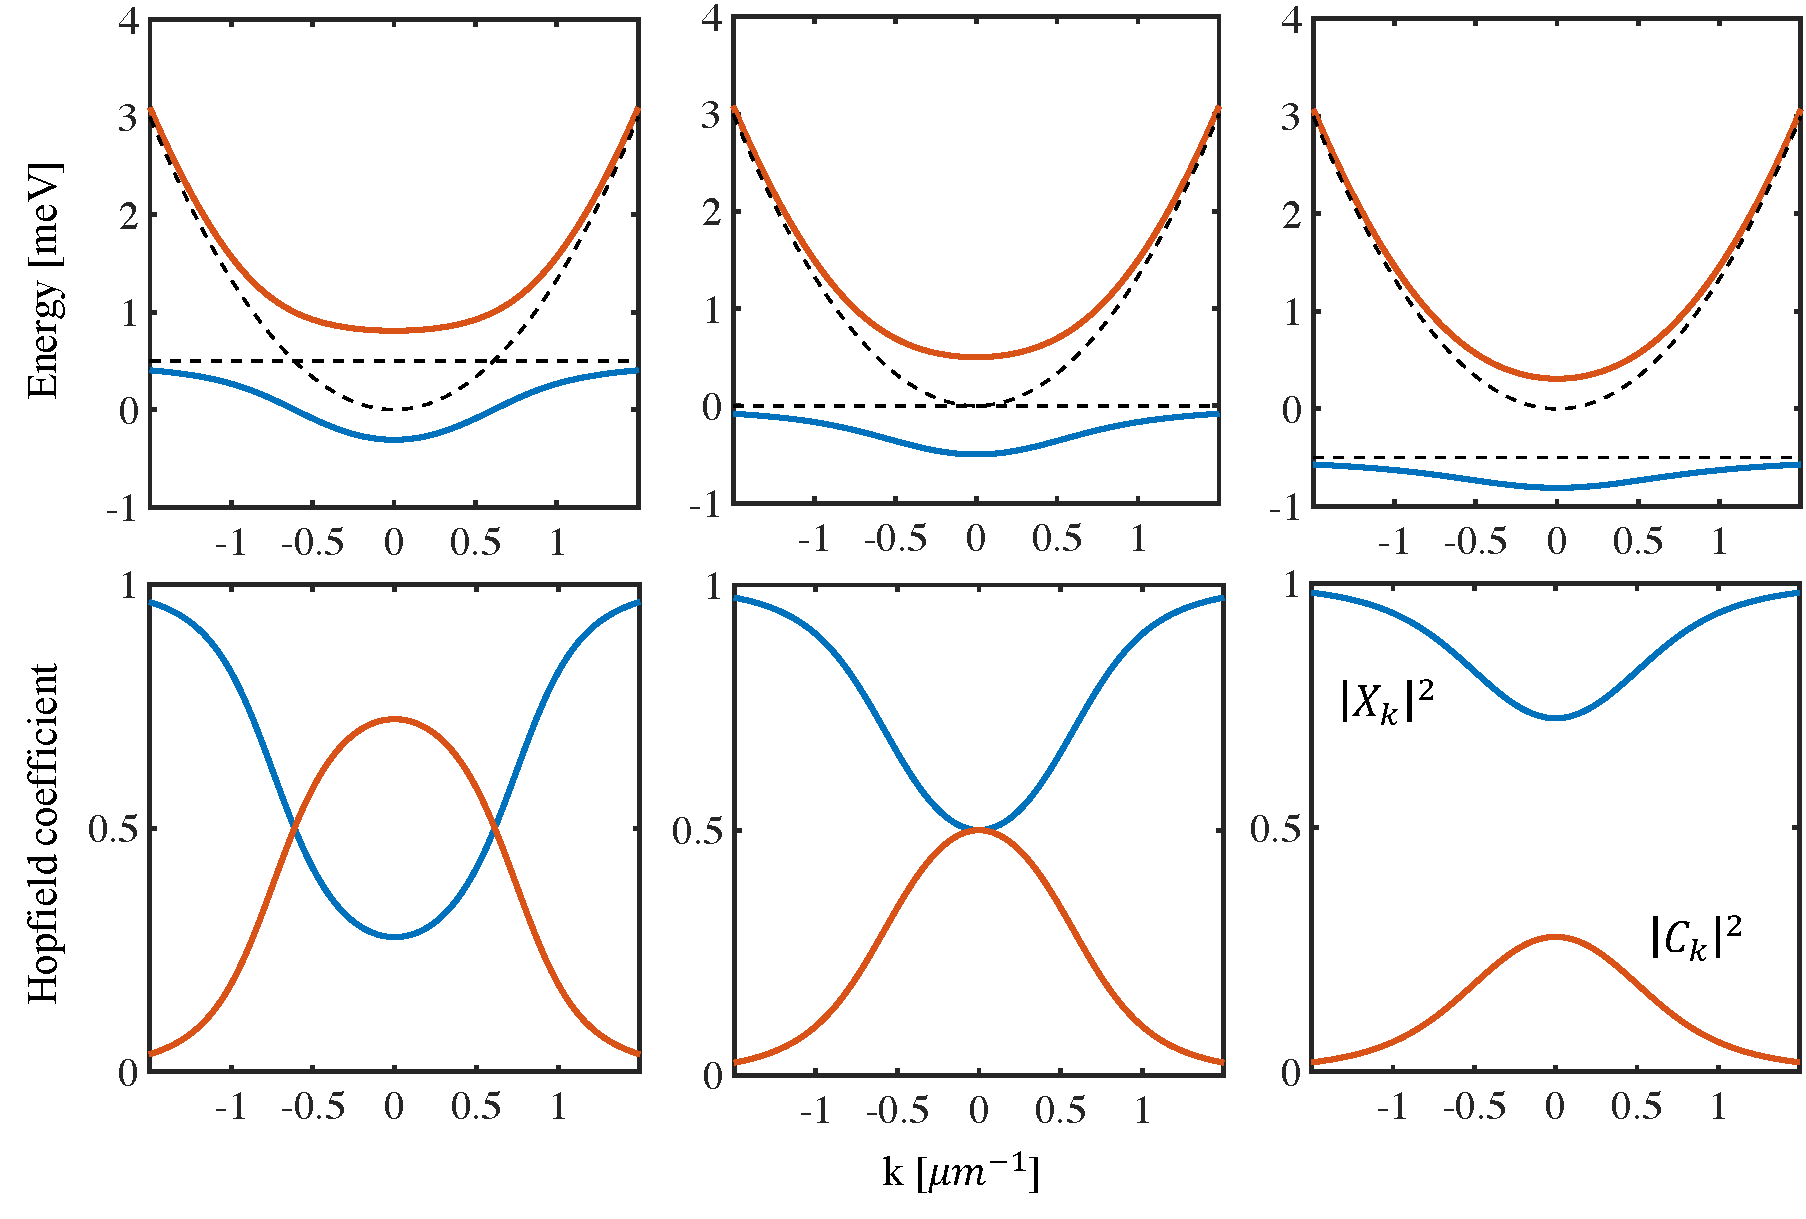
\includegraphics[width=0.65\linewidth]{Fig/Ch1/hp_disp.pdf}
    \caption[Polariton dispersion with different detuning]{Upper panel: Polariton dispersion from left to right with negative, zero, and positive detuning. Dashed lines correspond to the bare exciton and cavity photon mode. Lower panel: Corresponding Hopfield coefficients for the lower-branch polariton.}
    \label{fig:Ch1_disp}
\end{figure}
%
%
%

The effective mass of a polariton is the harmonic mean of the effective mass of its exciton and cavity photon.
For the lower-branch polaritons, we have
%
\begin{equation}
    \frac{1}{m_{lp}} = \frac{\abs{X_\mathbf{k}^L}^2}{m_{ex}} + \frac{\abs{C_\mathbf{k}^L}^2}{m_{cp}}.
    \label{eq:Ch1_mass}
\end{equation}
Due to the fact that the effective mass of excitons is much larger than that of cavity photons, the lower-branch polaritons at $\mathbf{k} \sim 0$ can be approximated by
\begin{equation}
    m_{lp} \approx \frac{m_{cav}}{\abs{C_\mathbf{k}^L}^2},~ ~ ~\textrm{when}~ \mathbf{k} \sim 0.
\end{equation}
Usually, this means that $m_{cav} \sim 10^{-4}m_{ex}$, which gives a much higher critical condensation temperature for polaritons than for excitons by considering the formula for critical temperature~\cite{pítajevskíj2003bose}
\begin{equation}
    T_c = \left(\frac{n}{\zeta\left(3/2\right)}\right)^{2/3} \frac{2\pi\hbar^2}{mk_B} \approx 3.3125 \frac{\hbar^2 n^{2/3}}{mk_B},
    \label{eq:Ch1_t_c}
\end{equation}
where $n$ is the density of particle, $m$ is the mass of the particle and $\zeta$ is the Riemann zeta function.
Thus given the same particle density, the temperature required for polaritons to reach condensation is orders of magnitude higher than the temperature for excitons.

\subsection{Polariton decay}
% The lifetime of the polariton is due to the finite lifetime of cavity photon and QW exciton.
% Due to the finite lifetime of cavity photons and QW excitons, polariton have
Because the cavity photons can escape from the microcavity, which de-stabilizes the bound state between excitons and photons, polaritons have a finite lifetime.
Let us consider $\gamma_{cp}$ as the decay rate of the cavity photons due to leakage from imperfect DBRs and $\gamma_{ex}$ as the decay rate of the excitons.
Then the corresponding non-Hermitian Hamiltonian is
%
\begin{equation}
        H =
    \begin{pmatrix}
        \frac{\hbar^2 k^2}{2m_{cp}} - \mi\hbar\gamma_{cp} & \Omega \\
        \Omega &  \frac{\hbar^2 k^2}{2m_{ex}}-\mi\hbar\gamma_{ex} - \delta
    \end{pmatrix}.
    \label{eq:Ch1_lifetime}
\end{equation}
%
We consider two cases separately: the strong and weak coupling regimes.
The difference between strong and weak coupling depends on the coupling strength, $\Omega$, and the difference between the decay rates of the excitons and cavity photons, $\gamma_{cp} - \gamma_{ex}$.
For strong coupling regime, one has the condition such that $2\Omega \gg \hbar\left(\gamma_{cp}-\gamma_{ex} \right)$, which indicates that the excitation can coherently transfer between photon and exciton at least once.
%
\begin{figure}[ht]
    \centering
    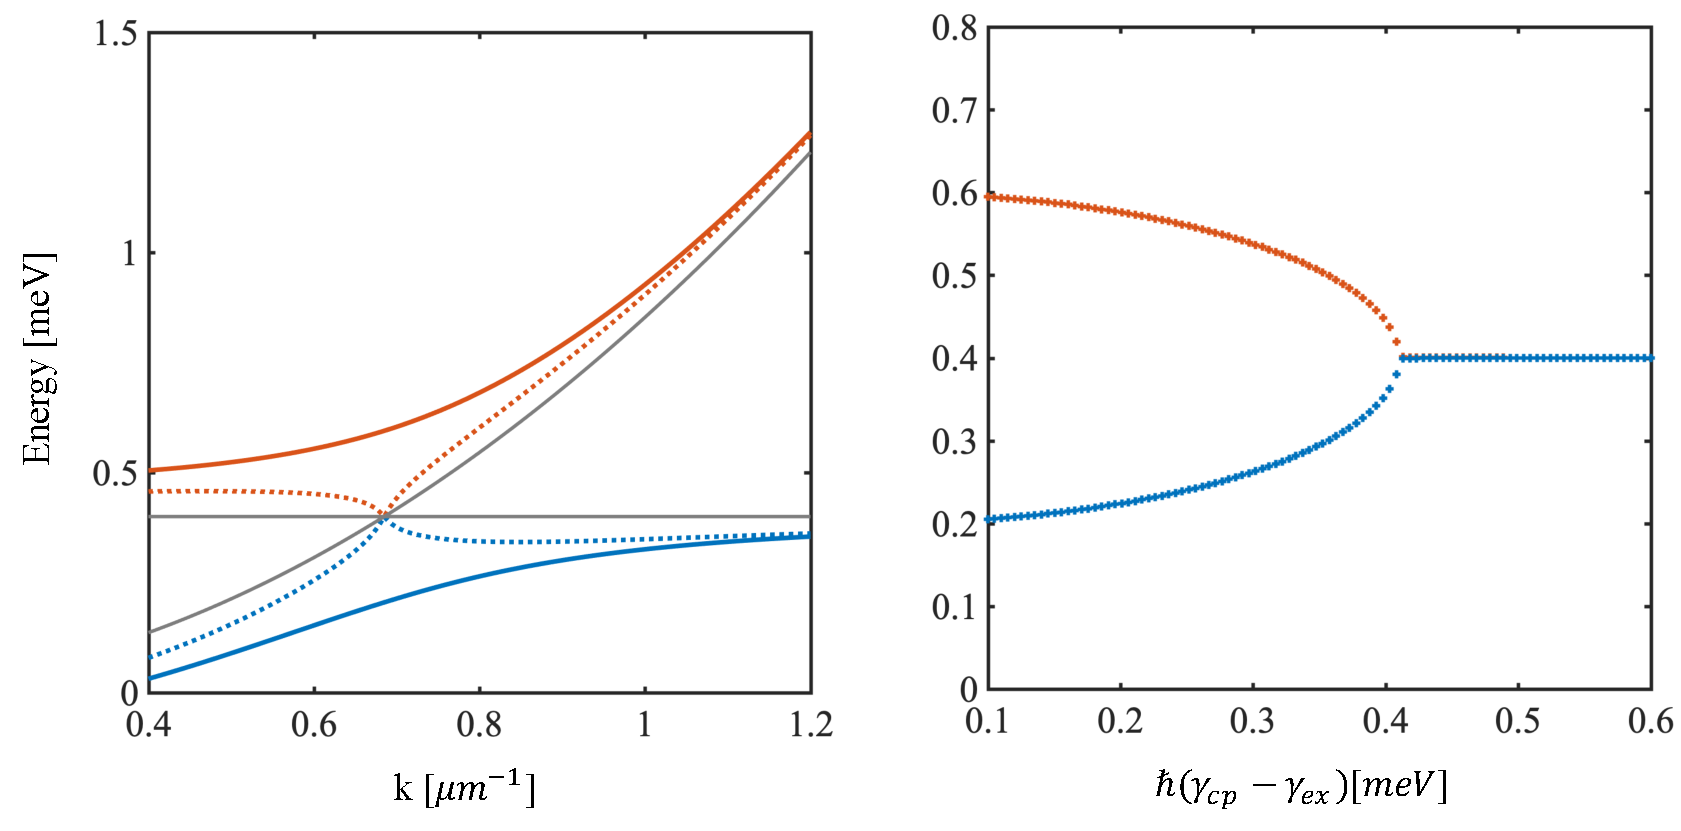
\includegraphics[width=0.65\textwidth]{Fig/Ch1/fig3.pdf}
    \caption[Polariton dispersion with decay]{Strong coupling regime (solid lines) and weak coupling regime (dotted lines) for the upper branch (red) and lower branch (blue). Left panel: Real parts of the eigenvalues. The grey lines show the uncoupled case for cavity photons and excitons. Right panel: The real part of eigenenergy for lower and upper branch of polariton at the point where the bare exciton and cavity photon cross as a function of decay rate difference between exciton and cavity photon.}
    \label{fig:Ch1_lifetime}
\end{figure}
%

In Fig.~\ref{fig:Ch1_lifetime} left panel, we plot the real part of the eigenvalues of Eq.~\eqref{eq:Ch1_lifetime} in different coupling regimes.
The parameters are chosen as follows: coupling strength $\Omega=0.2$~meV, detuning $\delta=0.4$~meV, exciton decay rate $\hbar\gamma_{ex} = 0.01$~meV, cavity photon decay rate $\hbar\gamma_{cp} = 0.1$~meV for the strong coupling case and $\hbar\gamma_{cp} = 0.41$~meV for thee weak coupling case.
In the right panel, we show the behaviour of the system gradually convert from the strong coupling to the weak coupling regime as increase the difference of the decay rate.
The energy gap is closed when $2\Omega=\hbar\left(\gamma_{cp}-\gamma_{ex}\right)$.

In the strong coupling limit, the two eigenvalues show an anticrossing behaviour and can be regarded as two polariton eigenmodes.
In polariton physics, we usually consider microcavities to have the following property: $\Omega \gg \hbar\gamma_{cp} \gg \hbar\gamma_{ex}$.
Then, Eq.~\eqref{eq:Ch1_eigv} can give us a nice approximation of the eigenenergies of the polariton.

\subsection{Exciton-polariton interaction}
One important difference between polaritons and cavity photons is the fact that polaritons can interact easily and directly with other particles due to their exciton component.
Polariton--polariton interaction can strongly affect the dynamics of the system, which leads to several fascinating nonlinear effects such as soliton behaviour and bistability.
Moreover, the excitonic part of polaritons can interact with excitations of surrounding lattices, which is known as interaction between polaritons and phonons.
By emitting and absorbing acoustic phonons, polaritons can transfer between different energy levels and reach BEC.

The interaction between exciton-polaritons is usually described by the following term
%
\begin{equation}
    \hat{H}_{pl-pl} = \frac{1}{2} \sum_{\mathbf{k,k^\prime ,q}} V_\mathbf{k,k^\prime,q} \hat{c}^\dagger_\mathbf{k+q}\hat{c}^\dagger_\mathbf{k^\prime -q}\hat{c}_\mathbf{k}\hat{c}_\mathbf{k^\prime},
    \label{eq:Ch1_pl-pl}
\end{equation}
%
where $V_\mathbf{k,k^\prime,q}$ accounts for the effective interaction strength between polaritons.
In the case when the momentum exchange is small, we can simplify the interaction as $V_\mathbf{k,k^\prime,0}\equiv V_{k}$.
One can further simplify the interaction term for a polariton system
\begin{equation}
    \label{eq:Ch1_pl-pl_detail}
    V_\mathbf{k} = \abs{X_k}^2\abs{X_k}^2 M_{ex},
\end{equation}
where $X_k$ is the Hopfield coefficient for polariton, and $M_{ex}$ is the exciton--exciton interaction which can be estimated by~\cite{Tassone:1999aa}
\begin{equation}
    \label{eq:Ch1_ex_ex}
    M_{ex} \approx 6 E_B \frac{a_B^2}{S}.
\end{equation}
Here $E_B$ is the exciton binding energy, $a_B$ is the exciton Bohr radius and $S$ is the sample surface.

The interaction between polaritons and phonons is given by~\cite{Deng:2010aa,Kavokin:2007aa}
%
\begin{equation}
    \hat{H}_{pl-ph} = \frac{1}{2} \sum_{\mathbf{k,q}}  V_{\mathbf{k,q}}^{ph} \hat{c}^\dagger_{\mathbf{k+q}}\hat{c}_\mathbf{k}\times \left( \hat{\mathscr{C}}_\mathbf{q,q_z} - \hat{\mathscr{C}}^\dagger_\mathbf{q,q_z} \right),
    \label{eq:Ch1_pl-ph}
\end{equation}
%
where $\hat{\mathscr{C}}_\mathbf{q,q_z}$ and $\hat{\mathscr{C}}_\mathbf{q,q_z}^\dagger$ are the phonon operators, $\mathbf{q_z}$ denotes the wavevector in the $z$ direction because the phonons are considered as three-dimensional particles unlike exciton-polaritons, and $V^{ph}_{\mathbf{k,q}}$ denotes the interaction strength between exciton-polaritons and phonons which is due to the interaction between excitons and phonons
\begin{equation}
    \label{eq:Ch1_ex_ph}
    V_{\mathbf{k,q}}^{ph}  = X_k^* X_\abs{\mathbf{k}+\mathbf{q}} \bra{k} \hat{H}_{ex-ph} \ket{k+q},
\end{equation}
where $X_k$ is the excitonic Hopfield coefficients of polariton.

\subsection{Exciton-polariton polarization}
Exciton-polaritons inherit pseudospin from the spin of their constituent excitons and cavity photons.
In the direction where the cavity grows, the total angular momentum of the electron in the conduction band is equal to $J_z^e=\pm \frac{1}{2}$, while that of the hole in the valance band is equal to $J_z^h = \pm \frac{1}{2}, \pm\frac{3}{2}$~\cite{Shelykh:2009aa}.
In the QW scenario, due to the confinement, the degeneracy in the different states is lifted.
Then the total angular momentum of an exciton in the ground state equals $J_z=\pm 1$ or $J_z =\pm 2$.
Moreover, because of the selection rules, the optical excitation on the excitons of state $J_z=\pm 2$ is strongly depressed, which means that they are not coupled with the photonic mode and do not form polaritons in the microcavity.
There are three main mechanisms of spin relaxation for excitons in semiconductors: (1) The Eliott--Yaffet mechanism~\cite{PhysRev.96.266} allows to transit between the light and dark exciton state, $J_z = \pm 1 \leftrightarrow J_z=\mp2$; (2) The D'yakonov--Perel mechanism~\cite{dyakonov1972spin} is caused by the spin-orbit interaction which also leads to the transition between $J_z = \pm 1 \leftrightarrow J_z=\mp2$; (3) The Bir--Aronov--Pikus mechanism~\cite{pikus1971exchange} involves the spin-flip exchange interaction of electrons and holes. Comparing to the two previous mechanisms, this mechanism is sufficiently enhanced in excitons~\cite{Maialle:1993aa}. This leads to the transition $J_z = +1 \leftrightarrow J_z=-1$.


% In order to describe the polarization of the polariton mode, we introduce the pseudospin formalism.
Let us introduce the pseudospin formalism that describes the polarization of the polariton mode.
Lower-branch polaritons at a given point $\mathbf{k}$ in reciprocal space can be described by a $2\times 2$ density matrix as
%
\begin{equation}
\rho_\mathbf{k} = N_\mathbf{k} \left[ \frac{\mathbf{I}}{2} + \mathbf{s}_\mathbf{k}\cdot \mathbf{\sigma}_\mathbf{k} \right],
\label{eq:Ch1_pseudospin}
\end{equation}
%
where $\mathbf{I}$ is the identity matrix, $\sigma_i$ is the Pauli matrix, $N_\mathbf{k}$ is the number of polaritons, and $\mathbf{s}_\mathbf{k}$ is the pseudospin of the polaritons.
In the strong coupling regime, these pseudospin components have a one-to-one correspondence to the Stokes parameters of the light emitted from the microcavity ~\cite{Kavokin:2004aa} with $\abs{\mathbf{s}}\leq \frac{1}{2}$ as shown in Fig.~\ref{fig:Ch1_pseudospin}.
In the general case, $s_z= \pm\frac{1}{2}$ denotes right- and left-circular polarizations, $s_x = \pm\frac{1}{2}$ denotes $X$- and $Y$-polarizations, and $s_y= \pm \frac{1}{2}$ denotes diagonal and anti-diagonal polarization.
Other points on the sphere represent the case of elliptical polarization.

%
\begin{figure}[ht]
    \centering
    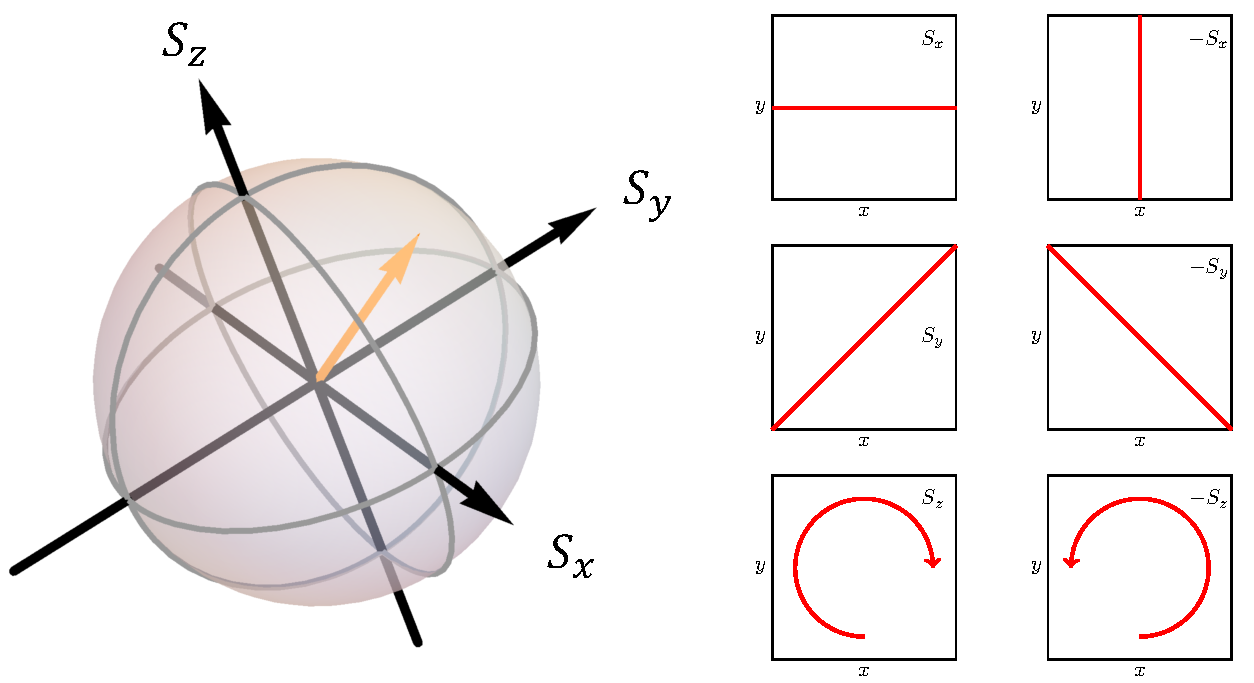
\includegraphics[width=0.65\textwidth]{Fig/Ch1/polarization_all.pdf}
    \caption[Pseudospin vector sphere]{Left: Pseudospin vector sphere. Right: Polarization of the $s_x$, $s_y$, and $s_z$ directions. The direction of the pseudospin vectors represent the polarization of the state. The north and south poles denote clockwise and anti-clockwise polarization, respectively, as shown in the bottom row of the right panel. The equator represents linear polarization, as shown in the upper two rows of the right panel.}
    \label{fig:Ch1_pseudospin}
\end{figure}
%

Experimentally, polaritons are usually excited by coherent or incoherent optical pumping, and thus polariton polarization is inherited from the exciting light.
However, the initial states of the pseudospin of the polaritons can evolve with respect to time under the effect of an external magnetic field and internal effective magnetic field.
The temporal evolution of the density matrix $\rho_\mathbf{k}$ is described by
%
\begin{equation}
\mi\hbar \frac{d \rho_\mathbf{k}}{dt} = \left[ H_\mathbf{k}, \rho_\mathbf{k}\right],
\label{eq:Ch1_evolution_spin}
\end{equation}
%
with the Hamiltonian reading
\begin{equation}
    H_\mathbf{k} = E_k + \frac{\hbar}{2}\left( \Delta^{eff}_\mathbf{k} \cdot \sigma_\mathbf{k} \right),
    \label{eq:Ch1_evolution_spin2}
\end{equation}
where $E_k$ is the bare dispersion of the polariton and $\Delta_\mathbf{k}^{eff}$ is the effective magnetic field.
In microcavities with cylindrical symmetry in the linear regime, the local effective magnetic field acting on the polariton pseudospin field is called transverse-electric-transverse-magnetic (TE-TM) splitting.
As it points out in~\cite{Maialle:1993aa}, because of the long-range exchange interaction between electrons and holes~\cite{pikus1971exchange}, exciton has different energy when the non-zero in-plane wavevector is parallel and perpendicular to its dipole moment orientation. Even though the magnitude can hardly exceed a few $\mu$eV for bare exciton, in microcavities this contribution can be greatly amplified due to the coupling to the cavity photon mode, which is also split in TE- and TM-light polarization~\cite{Panzarini:1999aa}. Yet another contribution to the polariton TE-TM splitting is the $k$-dependence of the exciton oscillator strength. The oscillator strength for TE excitons varies as a function of $\cos\theta$ and for TM excitons varies as $\cos^{-1}\theta$, where $\theta$ is the angle of light propagating in the cavity.
If one neglects the oscillator contribution, the TE-TM polariton splitting magnitude (for the lower-branch polariton) can be estimated by
%
\begin{equation}
    \Delta_\mathbf{k}^{eff} = \abs{X_\mathbf{k}}^2 \Delta_\mathbf{k}^{ex} + \abs{C_\mathbf{k}}^2\Delta_\mathbf{k}^{cp},
    \label{eq:Ch1_TE-TM_effect}
\end{equation}
%
where $X_\mathbf{k}$ and $C_\mathbf{k}$ are the Hopfield coefficients for excitons and cavity photons, respectively, and $\Delta_\mathbf{k}^{ex}$ and $\Delta_\mathbf{k}^{cp}$ are the TE-TM splitting for the bare excitons~\cite{Maialle:1993aa} and cavity photons~\cite{Panzarini:1999aa}, respectively.
The magnitude of the effective TE-TM splitting is highly sensitive to the detuning of the two modes and the center frequency of the cavity photons.
In some cases, one may achieve $\Delta_\mathbf{k}^{eff} \sim 10^2 \Delta_\mathbf{k}^{ex}$~\cite{Shelykh:2009aa}.

The formula for TE-TM splitting can be derived in the following way.
When we consider the polarization of the condensate, the equation of motion can be generally written as
%
\begin{equation}
    \mi\hbar \partial_t \vec{\psi}\left( \mathbf{r},t\right) = \frac{\delta H}{\delta \vec{\psi}^* \left( \mathbf{r},t\right)},
    \label{eq:Ch1_TE-TM_EOM}
\end{equation}
%
where the order parameter of the condensate $\vec{\psi}\left(\mathbf{r},t \right)$ is a complex 2D vector and a function of position in the microcavity plane ($\mathbf{r}$) and time ($t$).
Without losing any generality, we consider the Hamiltonian with only the kinetic term, as~\cite{Rubo2013}
%
\begin{equation}
    H = \int d\mathbf{r} \frac{\hbar^2}{2}\left( \frac{1}{m_l} \abs{\nabla \cdot \vec{\psi}}^2 + \frac{1}{m_t} \abs{\nabla \times \vec{\psi}}^2\right),
    \label{eq:Ch1_TE-TM_effect_mass}
\end{equation}
%
where $m_l$ and $m_t$ are the longitudinal and transverse effective mass of the polaritons, respectively.
The 2D vector of the order parameter can be rewritten in the circular polarization basis $\psi_\pm$, which gives
%
\begin{equation}
    \vec{\psi} =  \left[ \frac{\left(\mathbf{x}+\mi\mathbf{y} \right)}{\sqrt{2}}\psi_+ +\frac{\left( \mathbf{x}-\mi\mathbf{y}\right)}{\sqrt{2}}\psi_-\right].
    \label{eq:Ch1_linear_circular}
\end{equation}
%
Transferring from the Cartesian coordinate system $\{\mathbf{x},\mathbf{y}\} $ to circular components $\{ \mathbf{z},\mathbf{z}^*\}$, we have
%
\begin{equation}
    \mathbf{z} = \frac{\mathbf{x}+\mi\mathbf{y}}{\sqrt{2}}, ~ ~ ~ \mathbf{z}^* = \frac{\mathbf{x}-\mi\mathbf{y}}{\sqrt{2 }}.
    \label{eq:Ch1_basis}
\end{equation}
%
Given Eqs.~\eqref{eq:Ch1_linear_circular} and~\eqref{eq:Ch1_basis}, we can rewrite the cross product and inner product in this new coordinate as
%
\begin{equation}
    \nabla \cdot \vec{\psi} = \frac{\partial \psi_+}{\partial \mathbf{z}^*}+ \frac{\partial \psi_-}{\partial \mathbf{z}}, ~ ~ ~ \nabla \times \vec{\psi} = \frac{\partial \psi_+}{\partial \mathbf{z}^*} - \frac{\partial \psi_-}{\partial \mathbf{z}}.
    \label{eq:Ch1_derivative}
\end{equation}
%
Considering Eqs.~\eqref{eq:Ch1_TE-TM_EOM} and~\eqref{eq:Ch1_derivative} and with the technique of integrating by parts, we get
%
\begin{eqnarray}
    \mi\hbar \frac{\partial \psi_+}{\partial t} &= -\frac{\hbar^2}{m^*} \left(  \frac{\partial^2}{\partial \mathbf{z} \partial \mathbf{z}^*} \psi_+ + \gamma \frac{\partial^2 \psi_-}{\partial \mathbf{z}^2} \right),\\
    \mi\hbar \frac{\partial \psi_-}{\partial t} &= -\frac{\hbar^2}{m^*} \left(  \frac{\partial^2}{\partial \mathbf{z} \partial \mathbf{z}^*} \psi_- + \gamma \frac{\partial^2 \psi_+}{\partial \mathbf{z}^{*2}} \right),
    \label{eq:Ch1_TE_TM_Z}
\end{eqnarray}
where $\frac{1}{m^*}= \frac{1}{2}\left(\frac{1}{m_l}+\frac{1}{m_t}\right)$ and $\gamma = \frac{m_t-m_l}{m_t+m_l}$.
Changing the variables back to $\{ \mathbf{x},\mathbf{y}\}$ coordinates, we have
%
\begin{eqnarray}
        \mi\hbar \frac{\partial \psi_\pm}{\partial t} &= -\frac{\hbar^2}{2m^*} \left[ \left(\frac{\partial^2}{\partial \mathbf{x}^2}+ \frac{\partial^2}{\partial \mathbf{y}^2} \right) \psi_\pm + \gamma \left( \frac{\partial}{\partial \mathbf{x}} \mp \mi\frac{\partial}{\partial \mathbf{y}}\right)^2 \psi_\mp \right].
    \label{eq:Ch1_TE_TM_XY}
\end{eqnarray}
%
We can represent this equation in matrix form on the basis of polarization $\{\psi_+,\psi_-\}$ as
%
\begin{equation}
    E
    \begin{bmatrix}
    \psi_+ \\
    \psi_-
    \end{bmatrix}
    =
    \frac{\hbar^2}{2m^*}
    \begin{bmatrix}
    k_x^2 + k_y^2 & \gamma\left( k_x -\mi k_y\right)^2 \\
    \gamma\left( k_x +\mi k_y\right)^2 & k_x^2 + k_y^2
    \end{bmatrix}
    \begin{bmatrix}
     \psi_+ \\
    \psi_-
    \end{bmatrix}.
    \label{eq:Ch1_TE_TM_Eig}
\end{equation}
%
The result of the eigenvalue problem is shown in Fig.~\ref{fig:Ch1_TE_TM}.

%
\begin{figure}[ht]
    \centering
    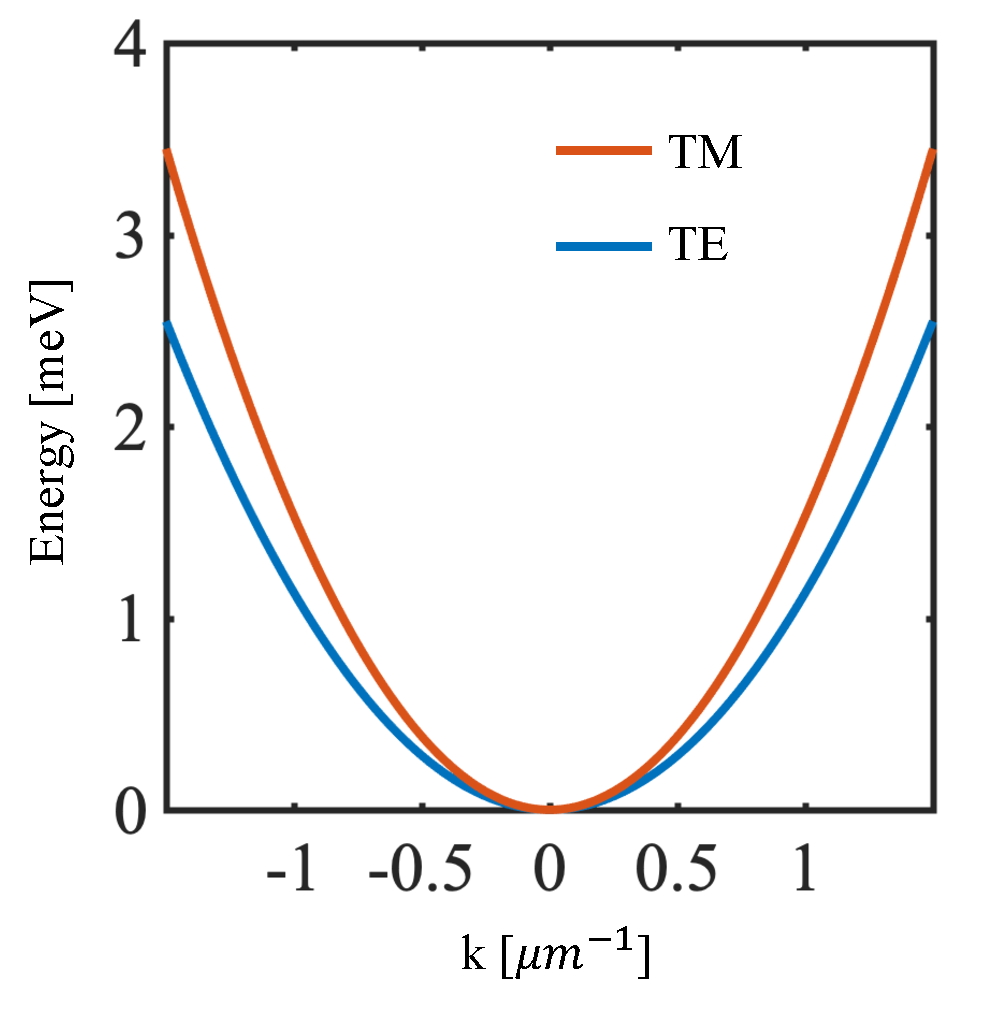
\includegraphics[width=0.35\textwidth]{Fig/Ch1/tetm.pdf}
    \caption[TE-TM Splitting]{Effective dispersion of TE and TM modes by solving Eq.~\eqref{eq:Ch1_TE_TM_Eig} with the following parameters:  $k_y = 0$ and $\gamma=0.2$~meV$\mu$m$^2$. }
    \label{fig:Ch1_TE_TM}
\end{figure}
%

Finally, we remark that in Eq.~\eqref{eq:Ch1_TE_TM_Eig}, we only consider the free dispersion case.
To describe more sophisticated problems, we need to consider extra terms like
%
\begin{equation}
    \mathcal{H} = H - \mu n + \mathcal{H}_{int} + \mathcal{H}^\prime,
    \label{eq:Ch1_TE_TM_extra}
\end{equation}
%
where $H$ is from Eq.~\eqref{eq:Ch1_TE-TM_effect_mass}, $\mu$ is the chemical potential, $n=\vec{\psi}^* \cdot \vec{\psi}$ is the exciton-polariton density, $\mathcal{H}_{int}$ is the interaction between particles, and $\mathcal{H}^\prime$ stands for the other possible perturbations.


\section{Exciton-polariton condensation}\label{se:CH1_EP-BEC}
In this section, we will first discuss the basic concepts of Bose--Einstein condensation and the experimental evidence of exciton-polariton condensation.
Then we will introduce the methods applied in the study of exciton-polariton condensation.

%There are several theoretical methods applied in the studying of polariton condensation.
%One noticeable method is called the semi-classical Boltzmann rate equation to describe the polariton kinetics in decades before ~\cite{Kavokin:2004aa,Tassone:1997aa,Tassone:1999aa,Ciuti:1998aa,Malpuech:2002aa,Porras:2002aa,Doan:2005aa}.
%The numerical simulation based on this theory give us a chance to understand the interaction of polariton, the relaxation of the polariton:

\subsection{Bose--Einstein condensation}
In quantum mechanics, bosons are particles that follow the Bose–Einstein statistics.
One important feature of bosons is that they are allowed to accumulate in a single degenerate quantum state.
According to Bose--Einstein statistics, at absolute zero, all particles should remain in their ground state.
Historically, in 1925, S. Bose~\cite{Bose:1924aa} and A. Einstein~\cite{Einstein:2006aa} proposed that a new phase transition should occur for non-interacting bosons at low temperature.
For many years, Bose--Einstein condensates were unreachable due to technological limits in cooling down the particles to their critical temperature.
Finally, in 1995, the first experimental observation of BEC was made and was later awarded the Nobel prize~\cite{Anderson:1995aa}.

Theoretically, BEC is a phase transition characterized by the macroscopic occupation of particles in their ground states.
Such a phase transition happens when the order parameter, i.e. chemical potential, becomes zero.

Let us consider $N$ non-interacting bosons at temperature $T$ in volume $L^d$, where $L$ is the system size and $d$ is the dimension of the system.
Then the distribution of the particles is given by
%
\begin{equation}
    f_B\left( \mathbf{k} ,T, \mu \right) = \frac{1}{\exp\left( \frac{E\left( \mathbf{k}\right) -\mu}{k_B T}\right)-1},
    \label{eq:Ch1_BEC_statistics}
\end{equation}
where $\mathbf{k}$ is the wavevector, $E\left( \mathbf{k}\right)$ is the particle dispersion (with $E\left(0\right)=0$), $k_B$ is the Boltzmann constant, and $\mu$ is the chemical potential ($\mu <0$).

%To add a particle to the system, one need extra energy $-\mu$.
%The value of $\mu$ is given by the normalization condition for the fixed total number of particles $N$,
For a fixed number of particles, in the normalization condition, we have
%
\begin{equation}
    N\left( T,\mu \right) = \frac{1}{\exp\left( -\frac{\mu}{k_B T}\right)-1} + \sum_{\mathbf{k}\neq 0} f_B \left( \mathbf{k},T,\mu\right),
    \label{eq:Ch1_BEC_distribtion}
\end{equation}
%
where we separate the particles in ground ($\mathbf{k}=0$) and excited ($\mathbf{k}\neq 0$) states.
In the thermodynamic limit, we can replace the summation with an integral and get the total particle density by
%
\begin{equation}
    n\left( T, \mu \right) = \lim _{L\to +\infty} \frac{N\left(T,\mu \right)}{L^d} = n_0 + \frac{1}{\left( 2\pi\right)^d} \int_0^{+\infty} f_B \left( \mathbf{k},T,\mu \right) d^d k,
    \label{eq:Ch1_BEC_density}
\end{equation}
with the ground state density,
%
\begin{equation}
    n_0 \left( T,\mu \right) = \lim_{L\to +\infty} \frac{1}{L^d} \frac{1}{\exp\left( -\frac{\mu}{k_B T} \right)-1}.
    \label{eq:Ch1_BEC_density0}
\end{equation}
When $\mu \neq 0$, the ground state density goes to zero.
The integral part of Eq.~\eqref{eq:Ch1_BEC_density} increases as the chemical potential $\mu$ approaches zero from negative infinity.
This means that if one increases the particle density ($n$) in the system, the chemical potential ($\mu$) will also increase.
The system reaches its critical density as follows,
%
\begin{equation}
    n_c\left(T\right) = \lim_{\mu \to 0} \frac{1}{\left( 2\pi \right)^d} \int_{0}^{+\infty} f_B \left( \mathbf{k},T \right)d^d k.
    \label{eq:Ch_1_critical_density}
\end{equation}
This integral can be calculated analytically in the parabolic dispersion case, which is $E\left(\mathbf{k}\right) = \frac{\hbar^2 k^2}{2m}$.
The result converges for $d>2$ and diverges for $d \leq 2$;
this means that if the system dimension is less than or equal to 2, the system can hold an infinite number of bosons while the chemical potential is non-zero.
Thus, BEC cannot happen in the $d \leq 2$ case.
When $d>2$, extra particles will collapse to the ground state when the system reaches its critical density.
This gives the density of the ground state as
%
\begin{equation}
    n_0\left(T\right) = n\left(T\right) -n_c\left(T\right).
    \label{eq:Ch1_groundstate_density}
\end{equation}
%
The appearance of the macroscopic occupation of the ground state indicates that BEC takes place.

In exciton-polariton physics, the particles are confined in the cavity, as shown in Fig.~\ref{fig:Ch1_cavity}.
This system can usually be regarded as a one-dimensional (1D) or 2D system.
From the previous discussion, we know that in 1D or 2D infinite homogeneous systems, Bose--Einstein condensate cannot exist in principle.
However, if the size of the system is finite, a quasi-condensation state is possible because of the cut off of the integral as discussed in~\cite{Bagnato:1991aa,Hohenberg:1967aa,PhysRevLett.17.1133}.

\subsection{BEC of exciton-polaritons}
The first experimental demonstration of Bose--Einstein condensation utilized dilute atomic gases; the first success was obtained in rubidium vapours~\cite{Anderson:1995aa} in 1995.
Following this early achievement, BEC based on exciton-polaritons was claimed~\cite{Kasprzak:2006aa} in 2006.
%
\begin{figure}[ht]
    \centering
    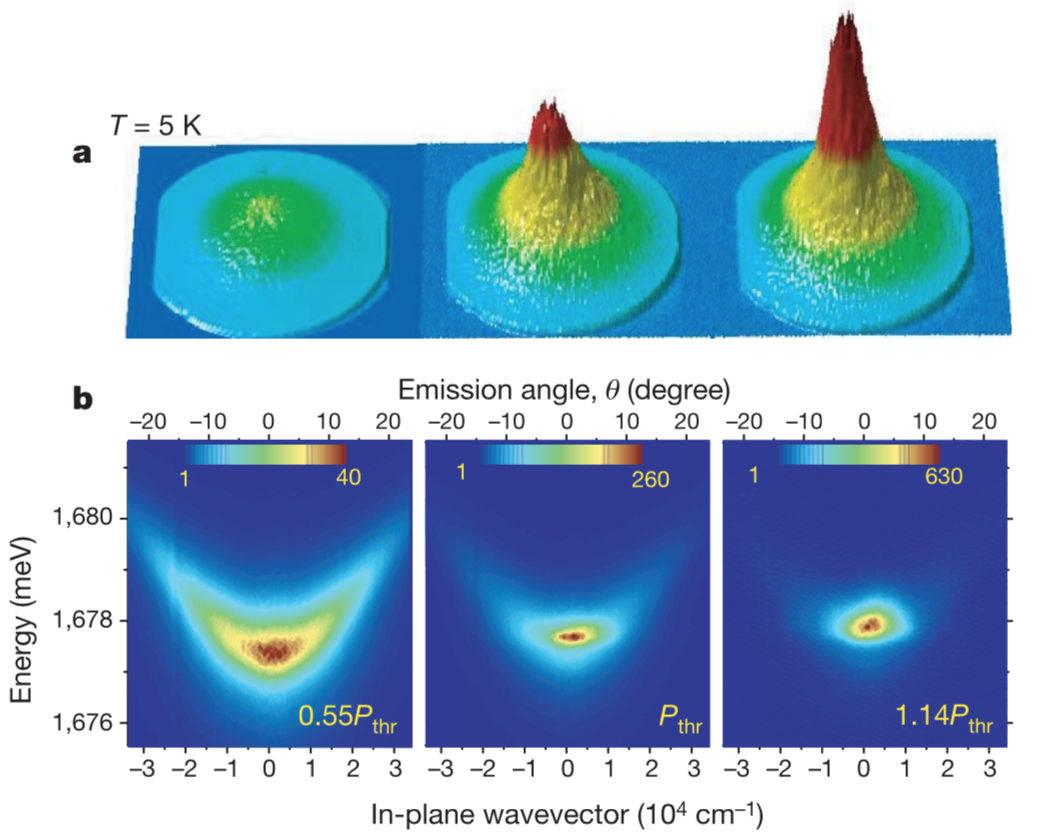
\includegraphics[width=0.65\textwidth]{Fig/Ch1/exp_BEC.png}
    \caption[Polaritons in BEC]{Bose--Einstein condensation of exciton-polaritons at $5$ K. (a) Pseudo-3D images of far-field emission with increasing pumping intensity. (b) Energy-resolved spectra results corresponding to (a). A narrowing of the particle distribution is shown at $k=0$ when the pumping is above the threshold. The figure is taken from~\cite{Kasprzak:2006aa}.}
    \label{fig:Ch1_exciton-polariton_BEC}
\end{figure}
%

In the work performed by Kasprzak et al.~\cite{Kasprzak:2006aa}, they applied a $\mathrm{CdTe}$/$\mathrm{CdMgTe}$-based microcavity at a temperature of $5$ K.
In Fig.~\ref{fig:Ch1_exciton-polariton_BEC}, they present particle density results based on the angular distribution of the spectrally integrated emissions.
From left to right, the pumping intensity increases gradually and crosses the pumping threshold.
As one can see in Fig.~\ref{fig:Ch1_exciton-polariton_BEC}(a), when the pumping is below the threshold (left panel), the far-field emission shows a smooth distribution centered around the ground state, i.e. $k=0$.
With increasing pumping intensity, from around the threshold (middle panel) to above the threshold (right panel), one can see that the emission from the ground state ($k=0$) increases sharply and becomes dominant.
This evidence reflects that the polaritons begin to macroscopically occupy the ground state when the pumping is above the threshold.
In Fig.~\ref{fig:Ch1_exciton-polariton_BEC}(b), the authors show the spectrum vs. angle-resolved results.
By increasing the pumping intensity, particle density at the ground state rises significantly.
One can also observe that the ground state energy also increases slightly due to particle interaction.

The previous experiment we discussed is based on a planar microcavity with no internal potential to confine the polaritons.
Instead of a potential profile of the microcavity, confinement in this case derives from the pumping because the size of the condensate strongly depends on the size of the pumping spot. However, with several modern techniques~\cite{Schneider:2017dq,Lai:2007aa,Cerda-Mendez:2010aa,Balili:2006aa} to modify the energy dispersion of cavity photons and QW excitons, one can achieve a strong trapping potential that can lead to single-mode or multi-mode exciton-polariton BEC.
Compared to the planar cavity case, the character of the BEC will be more obvious with the help of internal potential.
Through a periodic engineering of the microcavity, one can get a system with a particular potential as an analogue of different lattices to study the coherence properties and the interaction between different condensation modes.

One noticeable example was reported by Lai et al.~\cite{Lai:2007aa}.
In this work, they generated an array of trap potential around $U_0\approx200~\mu$eV by periodically applying thin metallic strips ($\mathrm{Au}$/$\mathrm{Ti}$) on the top of a microcavity, as shown in Fig.~\ref{fig:Ch1_periodic}(a).
%
\begin{figure}[ht]
    \centering
    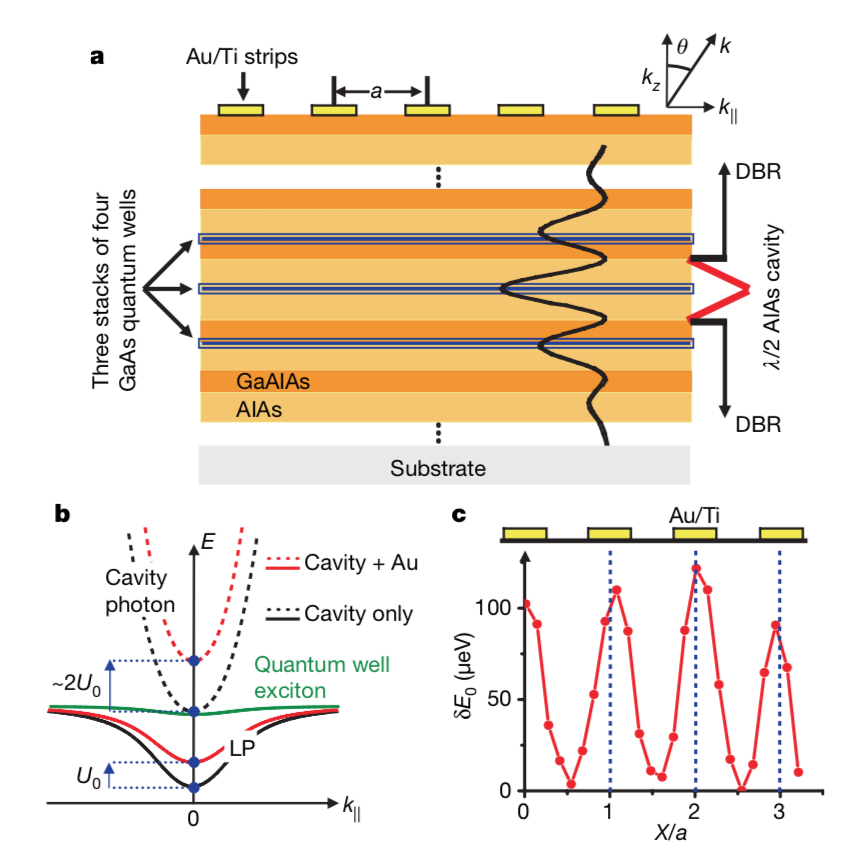
\includegraphics[width=0.65\textwidth]{Fig/Ch1/periodic.png}
    \caption[Polariton condensation in a periodic structure]{(a) Schematic of a cavity polariton array formed by placing periodic thin metallic strips ($\mathrm{Au}$/$\mathrm{Ti}$) on top of the cavity. (b) Dispersion for the cavity photon mode and lower-branch polariton mode. (c) Spatial energy modulation for the lower-branch polariton mode ($\delta E_0$) is detected from the position-dependent central energy of emission from lower-branch polaritons. The figure is taken from~\cite{Lai:2007aa}.}
    \label{fig:Ch1_periodic}
\end{figure}
%

Under the metallic layer mask, the resonance energy of the cavity photons is increased by $2U_0$ (at $k_\parallel=0$) compared to the case with a bare cavity, according to transfer-matrix calculation~\cite{Yeh:1988aa}.
As shown in Fig.~\ref{fig:Ch1_periodic}(b), when the cavity photons covered by the metallic layer couple with the excitons, the resulting lower-branch polaritons blueshift by about $U_0$ (at $k_\parallel=0$), compared to the case in which excitons are coupled with photons in the bare cavity region.
In Fig.~\ref{fig:Ch1_periodic}(c), the measured spatial modulation of the lower-branch polariton energy is shown, where the modulation is about $U_0/2\approx 100~\mu$eV. 
The energy difference between this measurement and the prediction in Fig.~\ref{fig:Ch1_periodic}(b) is due the limited spatial resolution of the optical detection system.

Then, the team excited the microcavity periodically masked by the metallic layers by a laser pulse near the QW exciton resonance.
With a large in-plane wave number of the laser pumping, one can make sure that the polariton coherence introduced by the laser is lost by the polariton-phonon scattering process before the polaritons reach the ground state at $k_\parallel=0$. 
This result is shown in Fig.~\ref{fig:Ch1_bandstructure}.
%
\begin{figure}[ht]
    \centering
    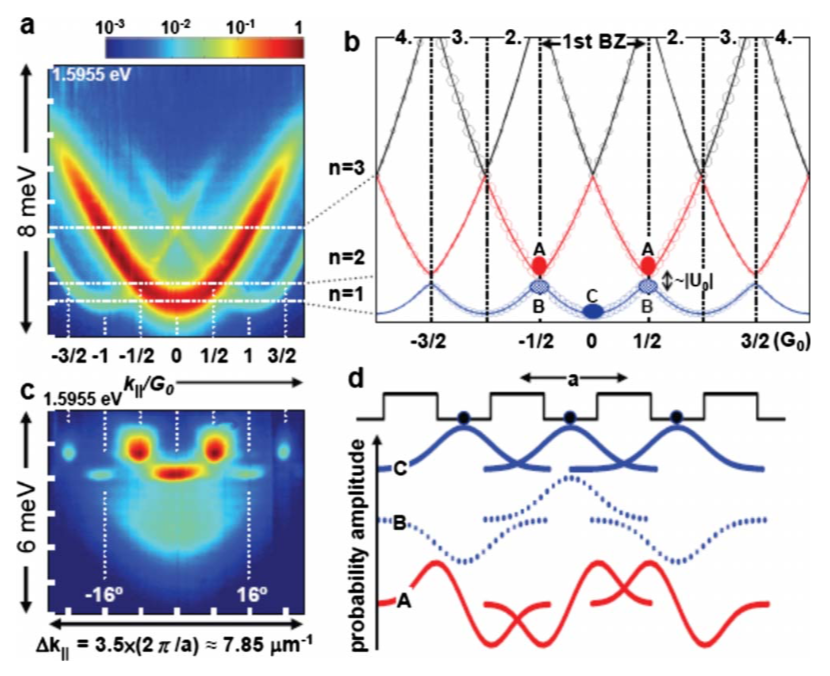
\includegraphics[width=0.65\textwidth]{Fig/Ch1/periodic2.png}
    \caption[Polariton band structure]{Energy-momentum dispersion and real space wavefunction of polaritons in a 1D array. (a) Time-integrated energy vs. in-plane momentum for the polariton array with detuning $E_{cav}\approx E_{exc}$ when the pumping is below the threshold. (b) Scheme of the band structure for the polariton array with lattice constant $a$. The gap between the first and second bands is about $\abs{U_0}\approx 200~\mu$ eV. (c) Energy vs. momentum of the polariton condensate array with detuning $E_{cav}-E_{exc}\approx 6$ meV when the pumping is above the threshold. (d) Scheme of the Bloch wavefunction for states A, B, and C labeled in (b). The figure is taken from~\cite{Lai:2007aa}.}
    \label{fig:Ch1_bandstructure}
\end{figure}
%

In Fig.~\ref{fig:Ch1_bandstructure}(a), the energy vs. in-plane momentum ($E$ vs. $k_\parallel$) dispersion relation for the 1D polariton array is shown.
In this situation, the detuning is close to zero, i.e. $E_{cav}\approx E_{exc}$, and the pumping is below the threshold.
To introduce the band structure for the polaritons in this array system, they applied a ``nearly free polariton" approximation in the presence of a periodic square-well potential.
Given a 1D periodic square potential $U\left(x\right)$ with a lattice constant, one can use Bloch theory to obtain the extended band structure, as presented in Fig.~\ref{fig:Ch1_bandstructure}(b).
The band gaps at the edge of the Brillouin zone due to the barrier potential are around $\abs{U_0}\approx 200~\mu$eV.
This result well reproduces the observed polariton energy dispersion in momentum space below the pumping threshold in Fig.~\ref{fig:Ch1_bandstructure}(a).
The absence of band gaps in the observed dispersion picture is due to the finite lifetime of the polaritons, which provides a large broadening of the emission lines (around $500~\mu$eV).

In Fig.~\ref{fig:Ch1_bandstructure}(c), the energy spectrum in momentum space is shown in the case with detuning $E_{cav}-E_{exc}\approx 6$ meV and pumping that is above the threshold.
In this situation, polariton emissions occur in two states with an energy difference of about $1$ meV.
Peaks of the emissions can be observed at $k_\parallel=0$ and $k_\parallel= \pm \frac{G_0}{2}$, and other weaker emissions can also be found at $k_\parallel = \pm G_0$ and $k_\parallel= \pm \frac{3G_0}{2}$, where $G_0=\frac{2\pi}{a}$ is the primitive reciprocal lattice vector.
The two states of emissions stand for the zero and $\pi$ states corresponding to $k_\parallel = 0,\pm G_0$ and $k_\parallel = \pm \frac{G_0}{2},\pm \frac{3G_0}{2}$, respectively.

A schematic of the spatial distribution based on the Bloch approach is drawn in Fig.~\ref{fig:Ch1_bandstructure}(d) for the states A, B, and C labeled in Fig.~\ref{fig:Ch1_bandstructure}(b).
The zero state labeled as C carries an s-like wave with a maximum amplitude in the potential wells and shares the identical phase between adjacent wells.
Meanwhile the states A and B at $k_\parallel=\pm \frac{G_0}{2}$ correspond to the $\pi$ state which has $\pi$ phase difference between adjacent wells.
However, compared to state A, state B is an unstable state, which can be examined by its different density distribution in real space.

The experimental realization in~\cite{Lai:2007aa} triggered a great scientific interest in investigating exciton-polaritons in different artificial lattices.
This is mainly because exciton-polariton gases under periodic lattice potential are a promising system to simulate many-body physics having relatively strong interaction, relatively small effective mass, and a variety of techniques to fabricate the lattice system.
To understand what happens in these many-body systems, we need to introduce some theoretical tools to describe system evolution in the next section.

\subsection{The driven-dissipative Gross--Pitaevskii equation}
In a previous subsection, we introduced an interaction term to describe the polariton-polariton collision in Eq.~\eqref{eq:Ch1_pl-pl}.
This interaction term makes the dynamics of the exciton-polaritons nontrivial and is responsible for a number of nonlinear and quantum effects.
%To solve the problem, one proper approach is the mean-field approximation.
% Considering the Hamiltonian of the exciton-polariton in condensate in real space,
%
% \begin{equation}
%     \hat{H} = \int \left(\frac{\hbar^2}{2m} \nabla \hat{\psi}^\dagger \nabla \hat{\psi}\right) dr + \frac{1}{2} \int \hat{\psi}^\dagger \hat{\psi}^{\prime \dagger} V\left(r^\prime -r\right) \hat{\psi}\hat{\psi}^\prime dr^\prime dr,
%     \label{eq:Ch1_Ham_GP}
% \end{equation}
%
% where $\hat{\psi} \equiv \hat{\psi}\left(r,t\right)$ is the field operator of exciton-polariton and $V\left(r^\prime -r\right)$ describe the strength of the two body interaction.
% In Heisenberg picture the equation of motion for operator $\hat{\psi}$ is the following,
% %
% \begin{eqnarray}
%   i\hbar \frac{\partial}{\partial t}\hat{\psi}\left(r,t\right) &=& \left[ \hat{\psi}\left(r,t\right),\hat{H}\right] \\
%   &=& \left( -\frac{\hbar^2 \nabla^2}{2m} + \int \hat{\psi}^\dagger\left(r^\prime,t\right)V\left(r^\prime -r \right) \hat{\psi}\left( r^\prime,t\right)d r^\prime\right) \hat{\psi} \left(r,t\right), \nonumber
%   \label{eq:Ch1_GP_eom}
% \end{eqnarray}
% %
% to get the second line of the equation of motion, we apply the integral by parts and the commutation relationship that: $\left[ \hat{\psi}\left(r,t\right), \hat{\psi}^\dagger\left(r^\prime,t\right) \right]= \delta\left(r-r^\prime\right)$.

% Transform the field operator into the momentum representation with this form:
% %
% \begin{equation}
%     \hat{\psi}\left(r\right) = \frac{1}{\sqrt{L}}\sum_k \hat{c}_k e^{i k \cdot r} 
%     \label{eq:Ch1_real_momentum}
% \end{equation}
% %
% where $\hat{c}_k$ is annihilation operator with momentum $k$, $L$ is the size of the system. 
% By inputting Eq.~\ref{eq:Ch1_real_momentum} into Eq.~\ref{eq:Ch1_Ham_GP}, we can get the Hamiltonian in momentum space,
% %
% \begin{equation}
%     \hat{H} = \sum_k \frac{\hbar^2k^2}{2m}\hat{c}_k^\dagger \hat{c}_k
%     + \frac{1}{2L} \sum_{p_1,p_2,q} V_q \hat{c}_{p_1+q}^\dagger \hat{c}_{p_2-q}^\dagger \hat{c}_{p_1} \hat{c}_{p_2}
%     \label{eq:Ch1_Ham_GP_P_space}
% \end{equation}
% %
% , where the $V_q = \frac{1}{\sqrt{L}}\int V\left(r\right) e^{ -i q\cdot r}dr$ is the Fourier transformation of the two body interaction $V\left(r\right)$.

% In the macroscopic scenario, when the properties of the condensate system are interested, only small momenta are involved in the system, so we can consider only the term $q=0$ for the interaction term as the approximation
% %
% \begin{equation}
%     V_0 = \alpha = \int V\left(r\right) dr.
%     \label{eq:Ch1_alpha}
% \end{equation}
% %
% Then the Hamiltonian in momentum space can be rewritten in the following form,
% %
% \begin{equation}
%     \hat{H} = \sum_k \frac{\hbar^2k^2}{2m} \hat{c}^\dagger_k \hat{c}_k + \frac{\alpha}{2L} \sum_{q,p_1,p_2} \hat{c}^\dagger_{p_1+q}\hat{c}^\dagger_{p_2-q}\hat{c}_{p_1}\hat{c}_{p_2}
%     \label{eq:Ch1_Mean_Hamil}
% \end{equation}

% According to the Bogoliubov prescription, for the zero momentum, i.e. the condensate part, we replace the operator $\hat{c}_0$ with a complex number,
% %
% \begin{equation}
%     c_0 \equiv \sqrt{N_0},
%     \label{eq:Ch1_q_0}
% \end{equation}
% %
% where $N_0$ is the number of the condensed particle.
% Meanwhile, the corresponding complex number field amplitude, so called order parameter $\psi_0\left(r,t\right)$, varies slowly over the distances comparable to the range of the inter-particle force.
% Thus we can replace the variable $r^\prime$ to $r$ in Eq.~\ref{eq:Ch1_GP_eom} and get the Gross-Pitaevskii equation,
% %
% \begin{equation}
%     i\hbar \frac{\partial }{\partial t}\psi_0\left(r,t\right) = \left( -\frac{\hbar^2 \nabla^2}{2m}  + \alpha \abs{\psi_0\left(r,t\right)}^2\right) \psi_0\left(r,t\right).
%     \label{eq:Ch1_Gross_Pitaevskii}
% \end{equation}
To investigate the many-body problem, one possible way is to apply the Hartee or mean-field approach and assume that the wavefunction is a symmetric product of a single-particle wavefunction.
Following the analysis in a text~\cite{Pethick:2002tn}, in a fully condensed situation, all the bosons are in the same single-particle state, and therefore we may write the $N$-particle wavefunction, $\Psi\left(\mathbf{r}_1,\mathbf{r}_2,...,\mathbf{r}_N\right)$, as
%
\begin{equation}
    \Psi\left(\mathbf{r}_1,\mathbf{r}_2,...,\mathbf{r}_N\right) = \prod_{i=1}^N \phi\left( \mathbf{r}_i\right).
    \label{eq:Ch1_many_wf}
\end{equation}
%
For each wavefunction in the single-particle state, we have the usual normalized condition
%
\begin{equation}
    \int d\mathbf{r}\abs{\phi\left(\mathbf{r}\right)}^2 = 1.
\end{equation}
%
To take interaction between the particles into account, we introduce an effective interaction term $U_0\delta\left( \mathbf{r}-\mathbf{r}^\prime\right)$.
Then the effective Hamiltonian may be written as
%
\begin{equation}
    H = \sum_{i=1}^N \left(\frac{\mathbf{p}_i^2}{2m} +V\left(\mathbf{r}_i\right) \right) + U_0 \sum_{i<j}\delta\left( \mathbf{r}_i - \mathbf{r}_j \right),
    \label{eq:Ch1_Ham_MP}
\end{equation}
%
where $V\left( \mathbf{r}\right)$ is the external potential.
The expectation value of the Hamiltonian in the state from Eq.~\eqref{eq:Ch1_many_wf} is given by
%
\begin{eqnarray}
        E &=& \bra{\Psi\left( \mathbf{r}_1,\mathbf{r}_2,...,\mathbf{r}_N \right)} H \ket{\Psi\left( \mathbf{r}_1,\mathbf{r}_2,...,\mathbf{r}_N \right)} \\ 
        &=& N \int d\mathbf{r} \left[ \frac{\hbar^2}{2m}\abs{\nabla \phi\left(\mathbf{r} \right)}^2 + V \left(\mathbf{r}\right) \abs{\phi\left(\mathbf{r}\right)}^2 + \frac{N-1}{2} U_0 \abs{\phi\left(\mathbf{r}\right)}^4\right]. \nonumber
        \label{eq:Ch1_Exp_Energy}
\end{eqnarray}
%
The factor before the interaction term, $C_N^2 =\frac{N\left(N-1\right)}{2}$, indicates all possible combinations of the interaction between two bosons in an $N$-particle system.

We introduce the concept of the wavefunction $\psi\left(\mathbf{r}\right)$ for the condensed state,
%
\begin{equation}
    \psi\left( \mathbf{r} \right) = \sqrt{N} \phi\left(\mathbf{r}\right),
    \label{eq:Ch1_order_parameter}
\end{equation}
%
as the order parameter.
With this new parameter, we can rewrite the energy of the system as
%
\begin{equation}
    E\left( \psi \right) = \int d\mathbf{r} \left[ \frac{\hbar^2}{2m}\abs{\nabla \psi\left(\mathbf{r} \right)}^2 + V \left(\mathbf{r}\right) \abs{\psi\left(\mathbf{r}\right)}^2 + \frac{1}{2} U_0 \abs{\psi\left(\mathbf{r}\right)}^4\right],
    \label{eq:Ch1_Exp_Energy_order}
\end{equation}
%
where we neglect the $N^{-1}$ term by assuming $N$ is large. 

As a next step, we minimize the energy in Eq.~\eqref{eq:Ch1_Exp_Energy_order} with respect to two independent variables $\psi\left(\mathbf{r}\right)$ and $\psi\left( \mathbf{r}\right)^*$ under the condition that the total number of particles is constant.
We first define the Lagrange multiplier as
%
\begin{equation}
    \mathcal{L}\left(\psi\left(\mathbf{r}\right),\psi^*\left(\mathbf{r}\right),\mu\right) = E\left(\psi\left(\mathbf{r}\right),\psi^*\left(\mathbf{r}\right)\right)-\mu \left(\int d\mathbf{r} \psi\left(\mathbf{r}\right) \psi^*\left(\mathbf{r}\right) -N \right),
    \label{eq:Ch1_Mulipler}
\end{equation}
%
and find the variation with respect to $\psi\left(\mathbf{r}\right)^*$ as
%
\begin{eqnarray}
        \delta_{\psi^*\left(\mathbf{r}\right)} \mathcal{L} &=& \delta_{\psi^*\left(\mathbf{r}\right)}\int d\mathbf{r} \left[ \frac{\hbar^2}{2m}\abs{\nabla \psi\left(\mathbf{r} \right)}^2 + V \left(\mathbf{r}\right) \abs{\psi\left(\mathbf{r}\right)}^2 + \frac{1}{2} U_0 \abs{\psi\left(\mathbf{r}\right)}^4 - \mu \psi\left(\mathbf{r}\right) \psi^*\left(\mathbf{r}\right)\right] \nonumber \\
        &=&  \int d\mathbf{r} \left[ \frac{\hbar^2}{2m}\nabla^2 \psi\left(\mathbf{r} \right) + V \left(\mathbf{r}\right) \psi\left(\mathbf{r}\right) +  U_0 \abs{\psi\left(\mathbf{r}\right)}^2 \psi\left(\mathbf{r}\right)- \mu \psi\left(\mathbf{r}\right) \right].
        \label{eq:Ch1_Mulipler2}
\end{eqnarray}
%
In order to get this result, we use the integrating by parts method and neglect the surface term by assuming that the size of the system is finite.
To get the extreme value for the energy with the constant number of particles constraint, we require that
%
\begin{equation}
     \delta_{\psi^*\left(\mathbf{r}\right)}\mathcal{L}\left(\psi\left(\mathbf{r}\right),\psi^*\left(\mathbf{r}\right),\mu\right) = 0.
\end{equation}
%
This gives us a time-independent Gross--Pitaevskii equation,
%
\begin{equation}
    -\frac{\hbar^2}{2m}\nabla^2 \psi\left(\mathbf{r}\right) + V\left(\mathbf{r}\right) \psi\left(\mathbf{r}\right) + U_0 \abs{\psi\left(\mathbf{r}\right)}^2 \psi\left(\mathbf{r}\right) = \mu \psi\left(\mathbf{r}\right),
    \label{eq:Ch1_Gross_Pitaevskii_t_independent}
\end{equation}
%
where $\mu$ is the chemical potential.
To get a time-dependent Gross--Pitaevskii equation, the stationary conditions $\psi\left(\mathbf{r},t\right)$ must develop in time as $e^{-\mi\mu t/\hbar}$, which gives
%
\begin{equation}
    \mi\hbar \frac{\partial \psi \left(\mathbf{r},t\right)}{\partial t} = -\frac{\hbar^2}{2m} \nabla^2 \psi\left(\mathbf{r},t \right) + V \left(\mathbf{r}\right) \psi\left(\mathbf{r},t\right) + U_0 \abs{\psi\left(\mathbf{r},t\right)}^2 \psi\left(\mathbf{r},t\right).
    \label{eq:Ch1_GP_time_dep}
\end{equation}
%

In exciton-polariton BEC, the number of particles in the condensate is not constant due to the finite lifetime of polaritons.
To maintain the condensation, one needs to introduce external pumping to the system in experiment.
Accordingly, we need to extend Eq.~\eqref{eq:Ch1_GP_time_dep} to a more generalized form to better describe the lower-branch polariton field.

If the Rabi frequency $\Omega$ is much larger than the other energy scales in the system, the generalized Gross--Pitaevskii equation for polaritons with a coherent pumping is~\cite{Carusotto:2013aa},
%
\begin{equation}
    \mi\hbar \frac{\partial}{\partial t} \psi\left(\mathbf{r},t\right) = \left[ -\frac{\hbar^2}{2m}\nabla^2 + V\left(\mathbf{r}\right) + \alpha \abs{\psi\left(\mathbf{r},t\right)}^2 -\frac{\mi \gamma}{2} \right] \psi\left(\mathbf{r},t\right) +  \mi P\left(\mathbf{r},t\right),
    \label{eq:Ch1_coherent_pump}
\end{equation}
%
where $\psi\left(\mathbf{r},t\right)$ represents the lower-branch polaritons, $\alpha$ is the interaction strength, $\gamma$ is the polariton decay, and $P\left(\mathbf{r},t\right)$ is the coherent pumping.

Equation~\eqref{eq:Ch1_coherent_pump} describes the case where the microcavity is driven by a coherent, quasi-resonant pump.
In this case, the microscopic details of the system are under control and one can develop an \textit{ab inito} description of the system~\cite{Carusotto:2013aa}.
However, another pumping scheme is widely applied in polariton physics, called incoherent pumping.
In incoherent pumping, the lower-branch polaritons do not inherit any information from the pumping source, such as phase or frequency, because of the relaxation process toward the bottom of the lower polariton branch.
Incoherent pumping usually pumps the system far above the bottom of the lower polariton branch by optical~\cite{PhysRevB.76.201305,Deng15318,PhysRevB.72.201301} or electrical means~\cite{Schneider:2013aa,PhysRevB.77.113303}.
The incoherent polaritons start to accumlate significantly in the bottleneck region in momentum space where the dispersion of polariton changes drastically.
The energy relaxation process toward the ground state is provided by the scattering of hot polaritons and phonons.
Due to the reducing of the density of state for lower polariton in the bottom region, the relaxation by phonon--polariton scattering is quite slow compared to polariton--polariton scattering in a strong enough pumping intensity.
For polariton--polariton collisions, two polaritons collide in the bottleneck region with each other.
One of the polaritons is scattered to the bottom of the lower polariton branch and the other one is scattered to the region where polariton is more excitonic.
Given the bosonic statistics of polaritons, this relaxation process turns out to be stimulated as soon as the density of polaritons at the bottom becomes unit.
This indicates that when the stimulation overcomes the losses, a macroscopic coherent population of polaritons starts to accumulate in the ground state i.e., the condensate appears.

In practice, to describe incoherent pumping, one should introduce an amplification term in the equation of motion Eq.~\eqref{eq:Ch1_GP_time_dep} to include the stimulated scattering into the condensate and an external rate equation to describe the polariton reservoir density

%
\begin{eqnarray}
        \mi\hbar \frac{\partial}{\partial t} \psi\left(\mathbf{r},t\right) &=& \left[ -\frac{\hbar^2}{2m}\nabla^2 + V\left(\mathbf{r}\right) + \alpha \abs{\psi\left(\mathbf{r},t\right)}^2 -\frac{\mi \gamma}{2} \right] \psi\left(\mathbf{r},t\right)\nonumber \\ &+& \frac{\mi}{2}R\eta_R\left(\mathbf{r},t\right) \psi\left(\mathbf{r},t\right),
        \label{eq:Ch1_inchoerent_pumping1}\\
        \frac{\partial}{\partial t} \eta_R\left(\mathbf{r},t\right) &=& I\left(\mathbf{r},t\right) - R \eta_R\left(\mathbf{r},t\right) \abs{\psi\left(\mathbf{r},t\right)}^2 - \gamma_R \eta_R \left(\mathbf{r},t\right).
        \label{eq:Ch1_inchoerent_pumping2}
\end{eqnarray}
%
Equation~\eqref{eq:Ch1_inchoerent_pumping2} describes the dynamics of the polariton reservoir density in the bottleneck region, $\eta_R\left(\mathbf{r},t\right)$, classically, where $I\left(\mathbf{r},t\right)$ is the intensity of the incoherent pumping, and $\gamma_R$ is the decay of the reservoir particles.
The reservoir is coupled to the condensed polaritons via the term $R\eta_R \left(\mathbf{r},t\right)\abs{\psi\left(\mathbf{r},t\right)}^2$, where $R$ is the phenomenological coupling strength between reservoir particles and condensed particles.

Equation~\eqref{eq:Ch1_coherent_pump} and Eqs.~\eqref{eq:Ch1_inchoerent_pumping1} \& \eqref{eq:Ch1_inchoerent_pumping2} are two important sets of equations to simulate the dynamics of exciton-polariton condensates.
By modifying the pumping terms and different shapes of the potential, we can realize various features of exciton-polariton systems, which we will discuss in the next several chapters.

\section{Outline of the thesis}
This thesis is organised as follows.
We discuss polariton condensation in simple artificial lattices in Chapter~\ref{CHTWO}.
Specifically, in Section~\ref{Ch2}, by engineering the potential of cavity photons and excitons separately, we get a non-trivial dispersion for polaritons in the ground state and study the dynamics of the system with an incoherent pumping model.
In Section~\ref{Ch3}, we consider an extended Gross--Pitaevskii equation with complex-valued potential and complex non-linearity to describe the gain and loss of polaritons in a 1D chain.
In this model, we find that condensation takes place in either the $0$- or $\pi$-state of the ground state, which is different from~\cite{Lai:2007aa}.
Next, in Chapter~\ref{CHTHREE}, we focus on the polariton in complex artificial lattices.
In Section~\ref{Ch4}, we provide a novel way to excite the compact localized condensation of exciton-polaritons in a Lieb lattice by Laguerre--Gaussian pumping and check the dynamics of the system.
In Section~\ref{Ch5}, we develop a method to generate topological edge states using a local magnetic field in a graphene lattice.
Following these treatments of exciton-polaritons in artificial lattices, in Chapter~\ref{Ch6}, we study the transport properties of 2D electron systems interacting with exciton or exciton-polariton condensates.
We show with this new type of interaction that the resistivity of the 2D material can be orders of magnitude higher than that from traditional phonon-electron interaction.
Finally, we conclude this thesis with a summary and further prospects related to the work in Chapter~\ref{Ch7}.
